\documentclass[12pt,a5paper]{article}

\usepackage[utf8]{inputenc}
\usepackage{graphicx}
\usepackage{tikz}
\usetikzlibrary{calc}
\usepackage{fix-cm}

\parindent=0pt

\usepackage[pages=some]{background}
\backgroundsetup{%
contents={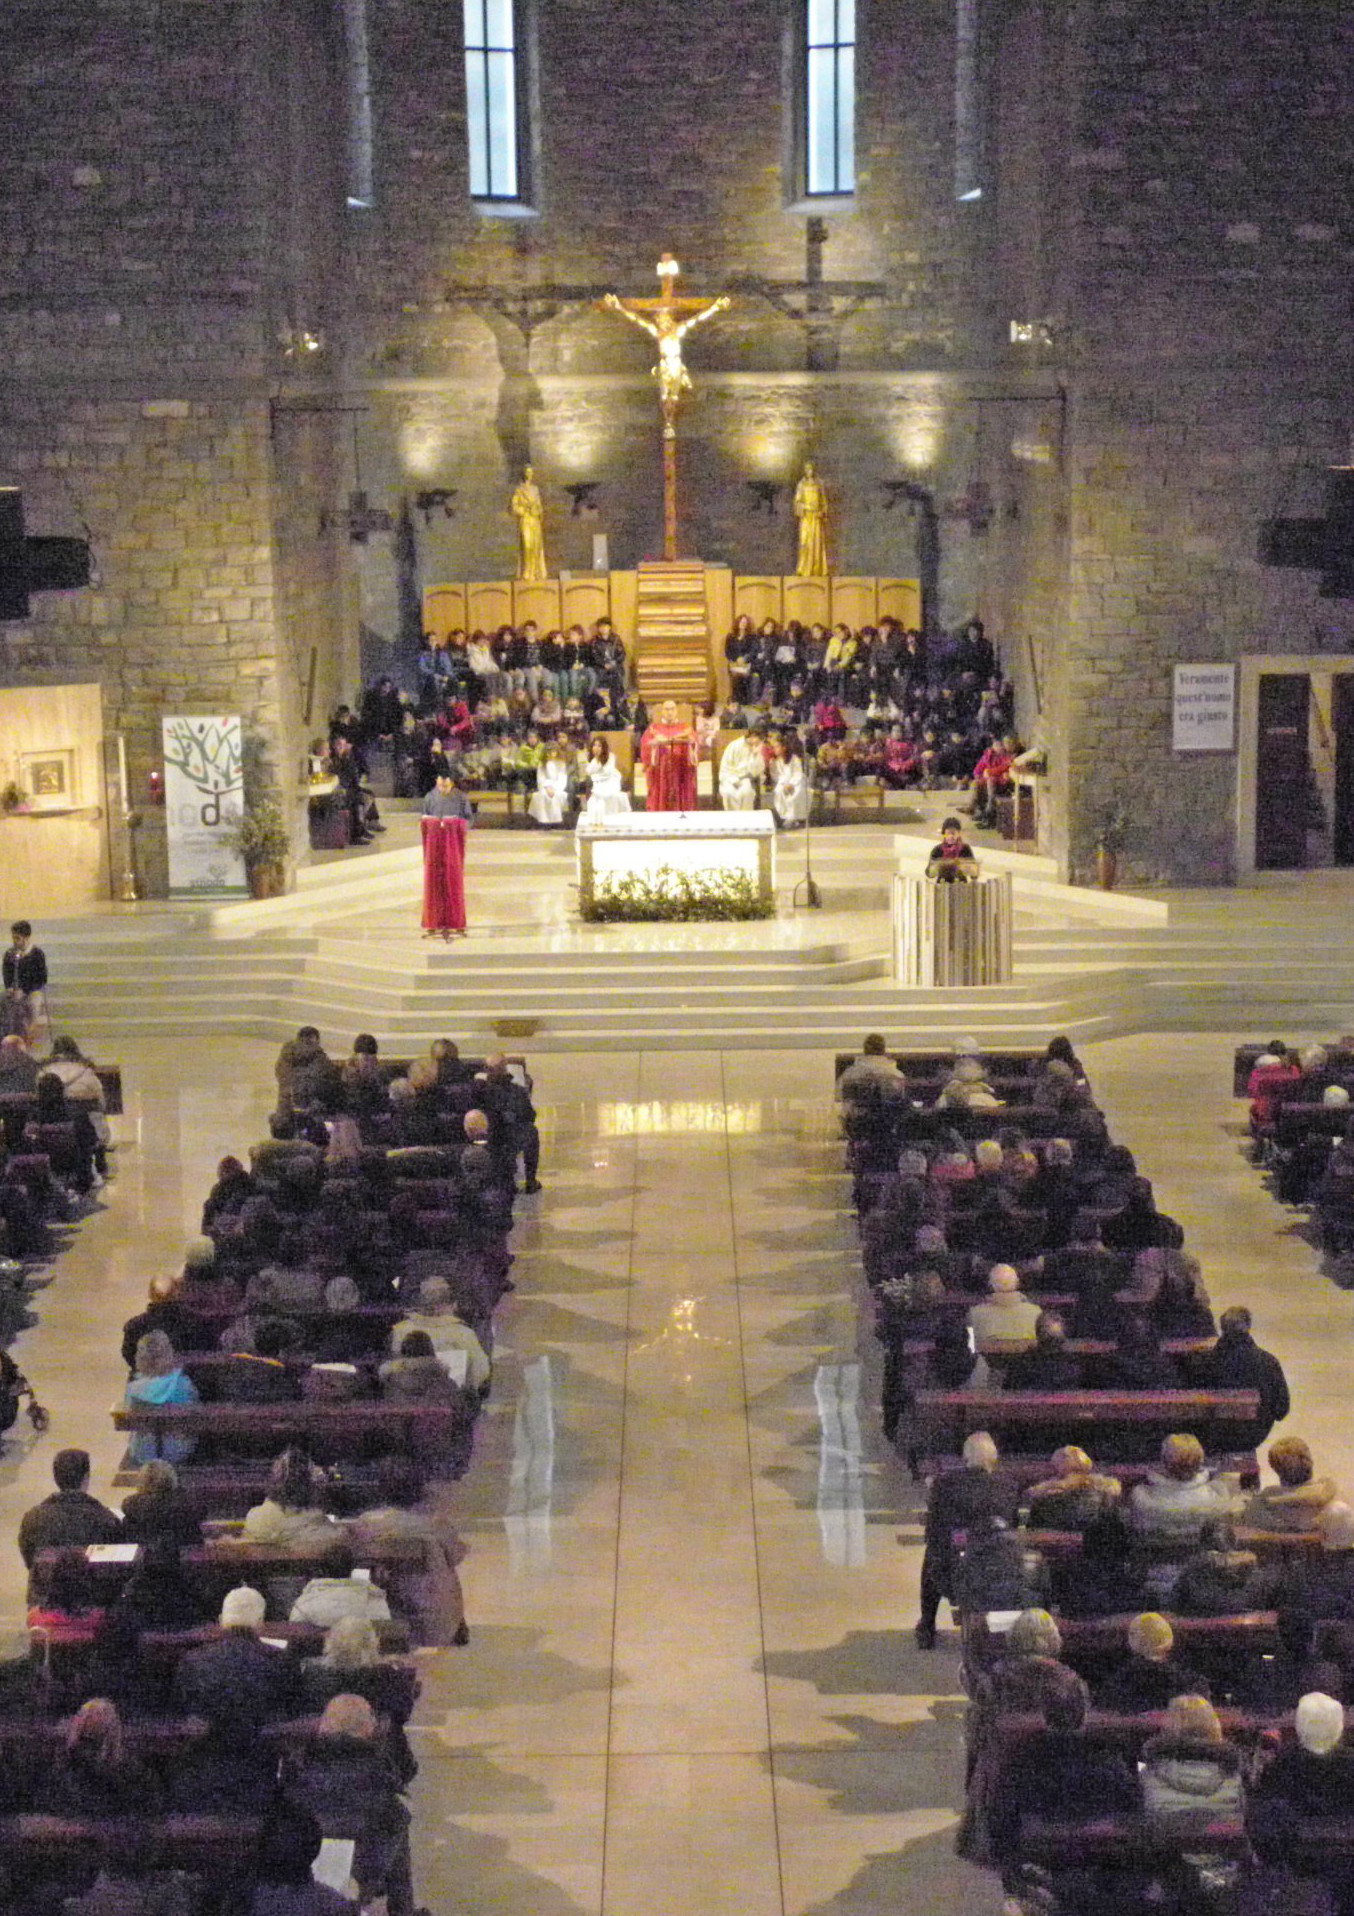
\includegraphics[width=\paperwidth,height=\paperheight]{chiesa}}, 
angle=0,
opacity=1.0,
scale=1
}

\begin{document}
\pagestyle{empty}
\BgThispage
\begin{tikzpicture}[remember picture, overlay]
\node[minimum width=\paperwidth, minimum height=6cm, outer sep=0pt, fill=white!30, fill opacity=0.6, text opacity=1, align=center] at (current page.center) {%
    \sffamily\Large PARROCCHIA di SAN FRANCESCO\\[10pt] \sffamily\huge TRIESTE\\[25pt]
    \fontsize{25}{25}\selectfont \bfseries 2015: 50 ANNI di VITA\\[25pt]
    \Large la comunità racconta\par%
};
\end{tikzpicture}

\end{document}  